\chapter{Concepts}
\label{ch:Concepts}

This chapter presents the concepts that are evaluated in the trade-off.
These concepts stem from a design option tree (DOT), which has been made using three subsystem DOTs.
Each concept will be briefly explained, and a sketch of each concept will be shown to clarify the concepts further.

\section{Design Option Tree}
\label{sec:DesignOptionTree}
It was chosen to perform a DOT on the main wing configuration, on the ground footprint reduction and on the propulsion configuration. The three preliminary DOTs can be found in \Cref{fig:DOTs_subsystems};
Afterwards, the three DOTs were combined into the final DOT, which is attached in the appendix.
From the final DOT, it can be concluded that the propulsion for the concepts has not yet been finalised, as it will be finalised during the detailed design of the vehicle.

\begin{figure}[H]
    \centering
    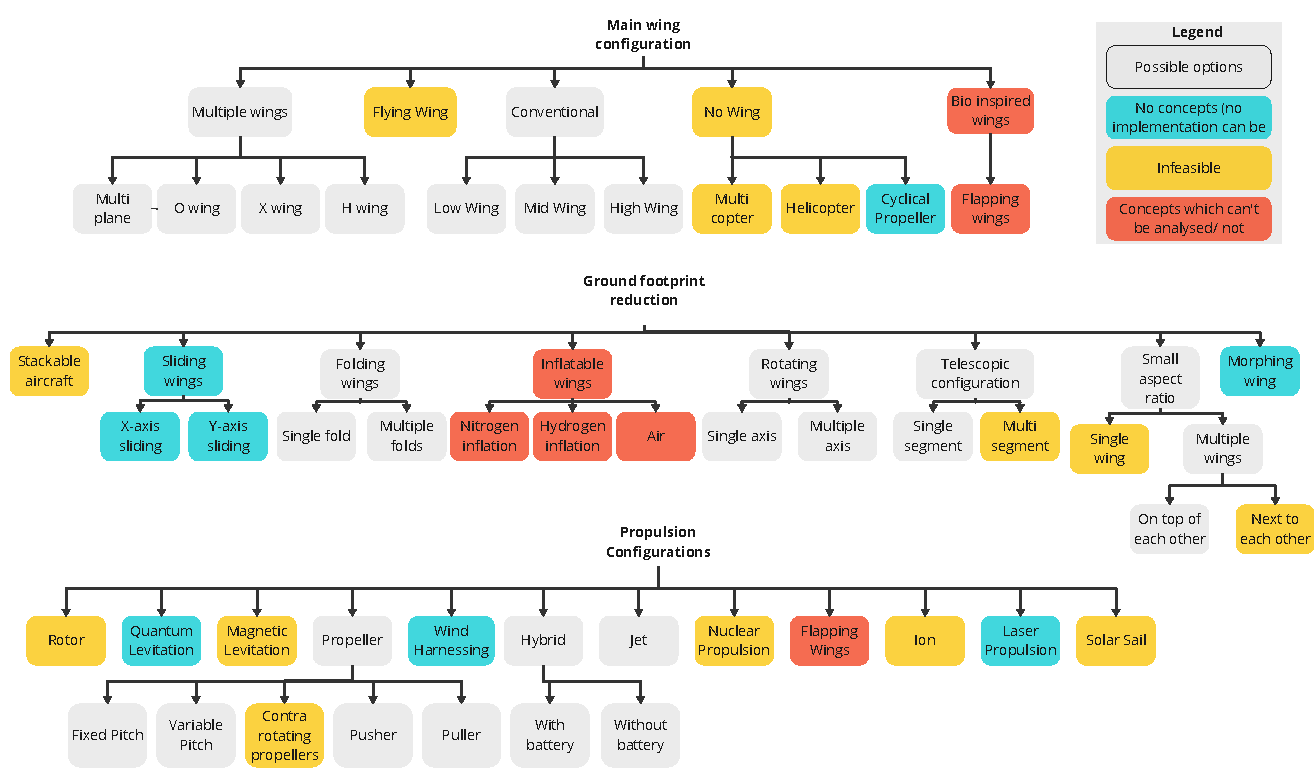
\includegraphics[width=1\linewidth]{figures/AE3200 DOT subsystems.pdf}
    \caption{Design option trees of subsystems}
    \label{fig:DOTs_subsystems}
\end{figure}




\section{Design Options}
\label{sec:DesignOptions}
Based on the final Design Option Tree present in the appendix, several concepts are identified as feasible and shall be analysed in the trade-off.

In \Cref{fig:ConceptC1.5} the \textit{Winged Rotorcraft} is shown.
The design features four rotatable propulsion units, two at the front and two at the back of the vehicle.
Additionally, the wing of the vehicle can be folded to stay within the ground footprint, while during the horizontal flight phase, the wing will be folded out to increase the lift-generating capabilities of the vehicle.

\Cref{fig:ConceptC2.1} shows the \textit{Rotating Wing}, this concept features four propulsion units that are fixed on the main wing.
The wing itself does rotate moreover, the wing rotates about multiple body axis of the vehicle.
While the hinge itself only has one axis of rotation.
During the horizontal flight phase, the wing is rotated in order to both produce lift and to \enquote{rotate} the propulsion units to produce thrust.
This concept is inspired by Pterodynamics\footnote{https://pterodynamics.com [Accessed on 17-05-2024]}.

Similarly to the \textit{Winged Rotorcraft} the \textit{Folding Wing}, shown in \Cref{fig:ConceptC2.6}, also features a folding wing.
The two front rotatable propulsion units are placed on the main wing of the vehicle, whereas the two units at the back are placed on the vertical tail.
During the horizontal flight phase the wing will be folded out to increase the lift generating capabilities of the vehicle.
Additionally, the engines on the main wing will have to be extended forward during the vertical flight phase.
Otherwise interference between the engine airflow and the wing surface would be present, this would reduce the engine efficiency and thus increase energy consumption.

Finally, \Cref{fig:ConceptC2.10} shows the \textit{Variable Skew Quad Plane}, this concept features five propulsion units.
Four propulsion units are used purely for the vertical flight phase, and one propulsion unit is used for the horizontal flight phase.
Additionally, this design features an oblique wing which is rotated during the horizontal flight phase to produce lift.
This concept is inspired by AEROGRID UAV\footnote{https://aerogriduav.com [Accessed on 17-05-2024]}.

\begin{figure}[h]
    \centering
    
\begin{subfigure}[b]{0.49\textwidth}
    \centering
    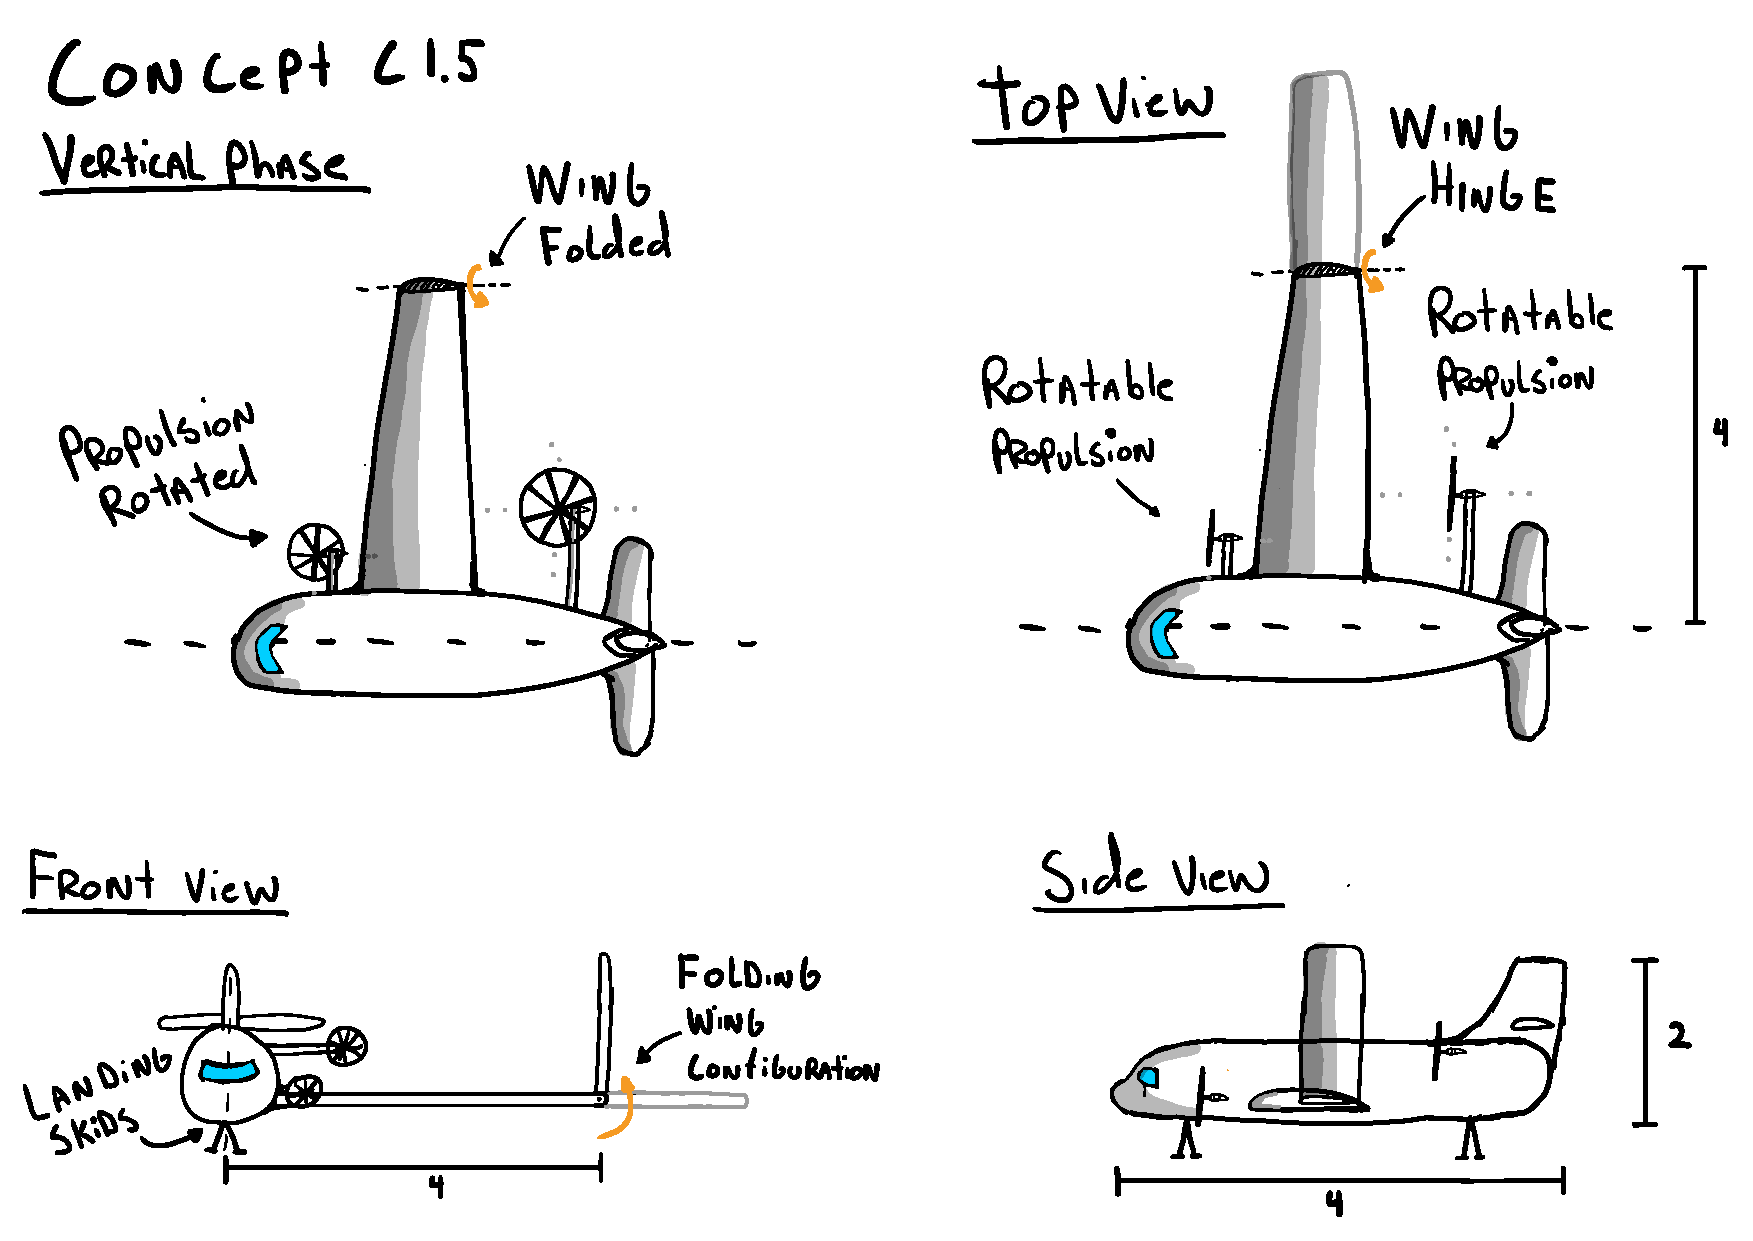
\includegraphics[width=1\linewidth]{figures/Concepts/Concept C1.5 v3.pdf}
    \caption{Concept \newtag{C1.5}\label{C:Winged-Rotorcraft}: Winged Rotorcraft}
    \label{fig:ConceptC1.5}
\end{subfigure}
\vrule
\begin{subfigure}[b]{0.49\textwidth}
    \centering
    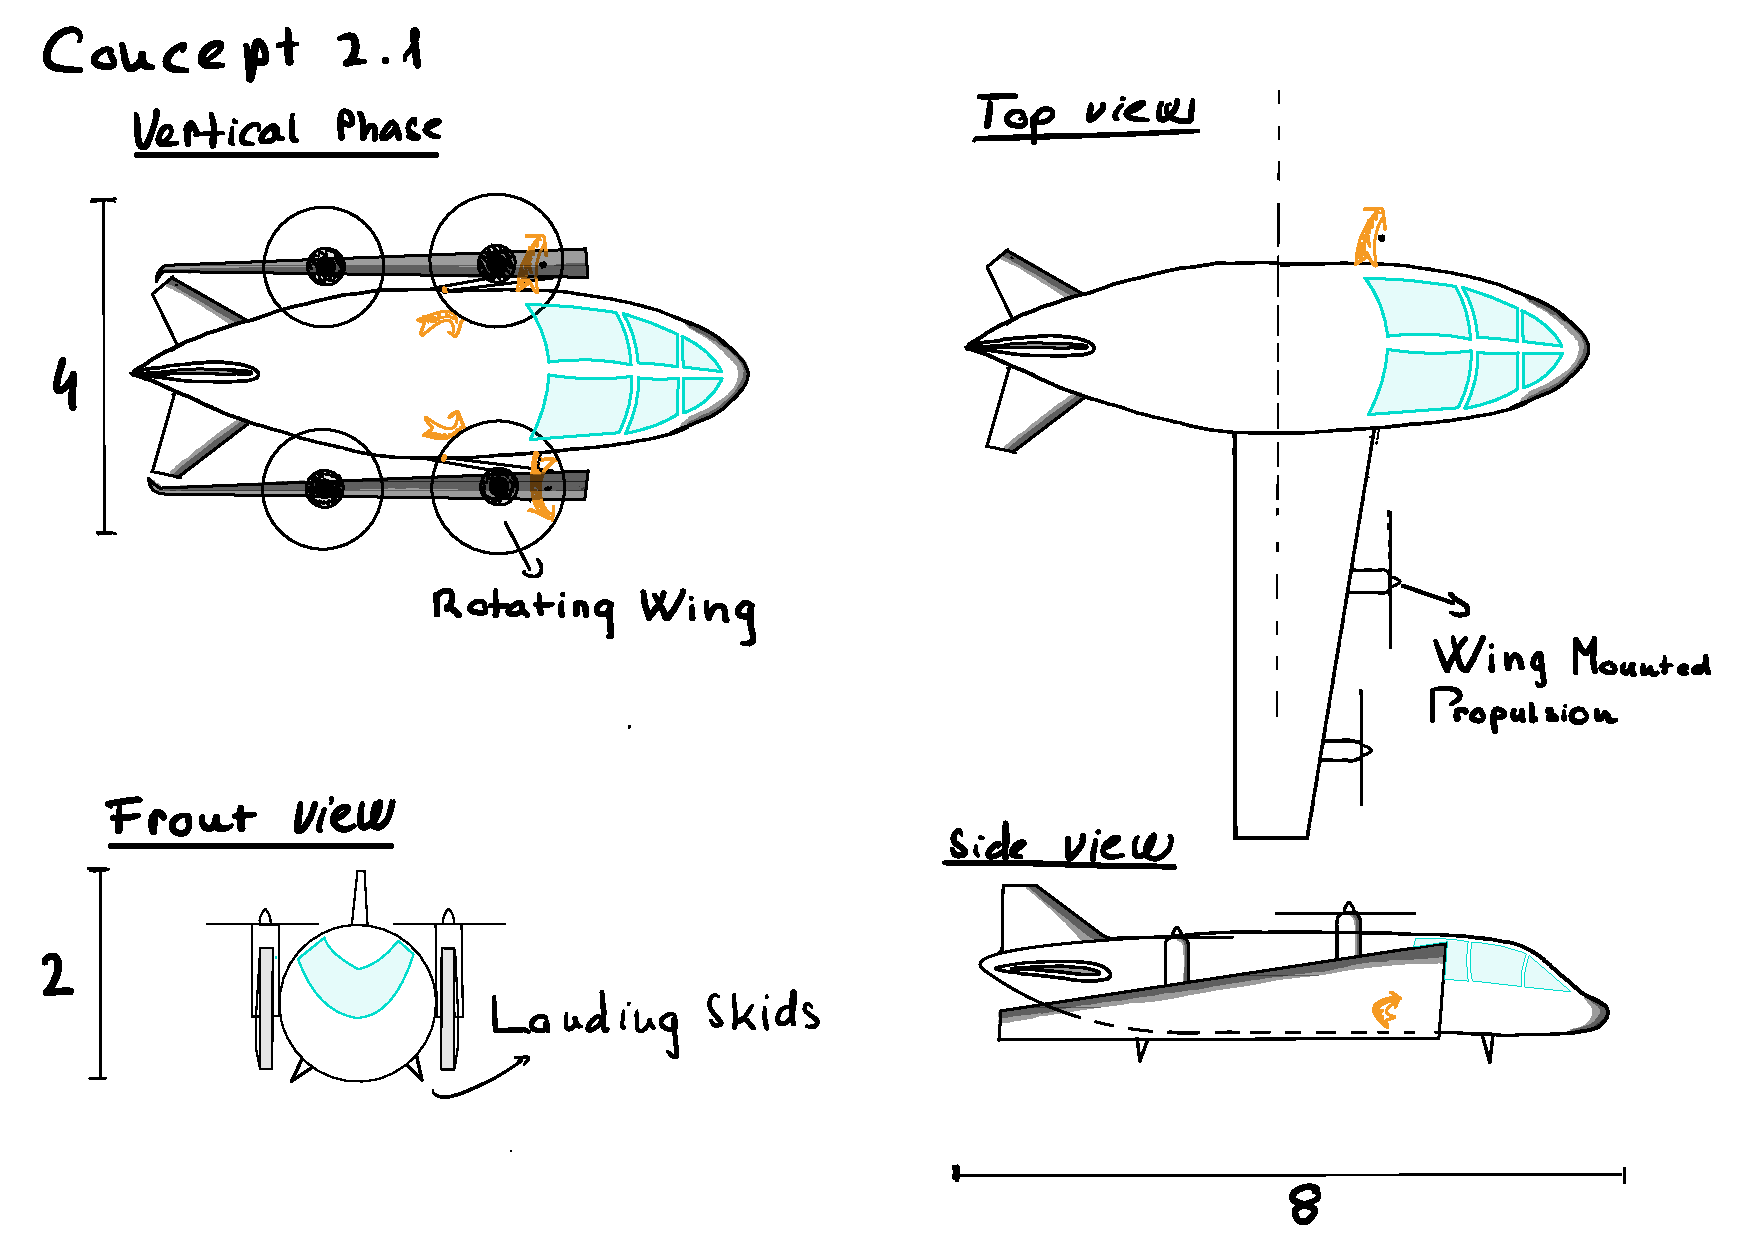
\includegraphics[width=1\linewidth]{figures/Concepts/Concept C2.1 v3.pdf}
    \caption{Concept \newtag{C2.1}\label{C:Rotating-Wing}: Rotating Wing}
    \label{fig:ConceptC2.1}
\end{subfigure}
\hrule
\begin{subfigure}[b]{0.49\textwidth}
    \centering
    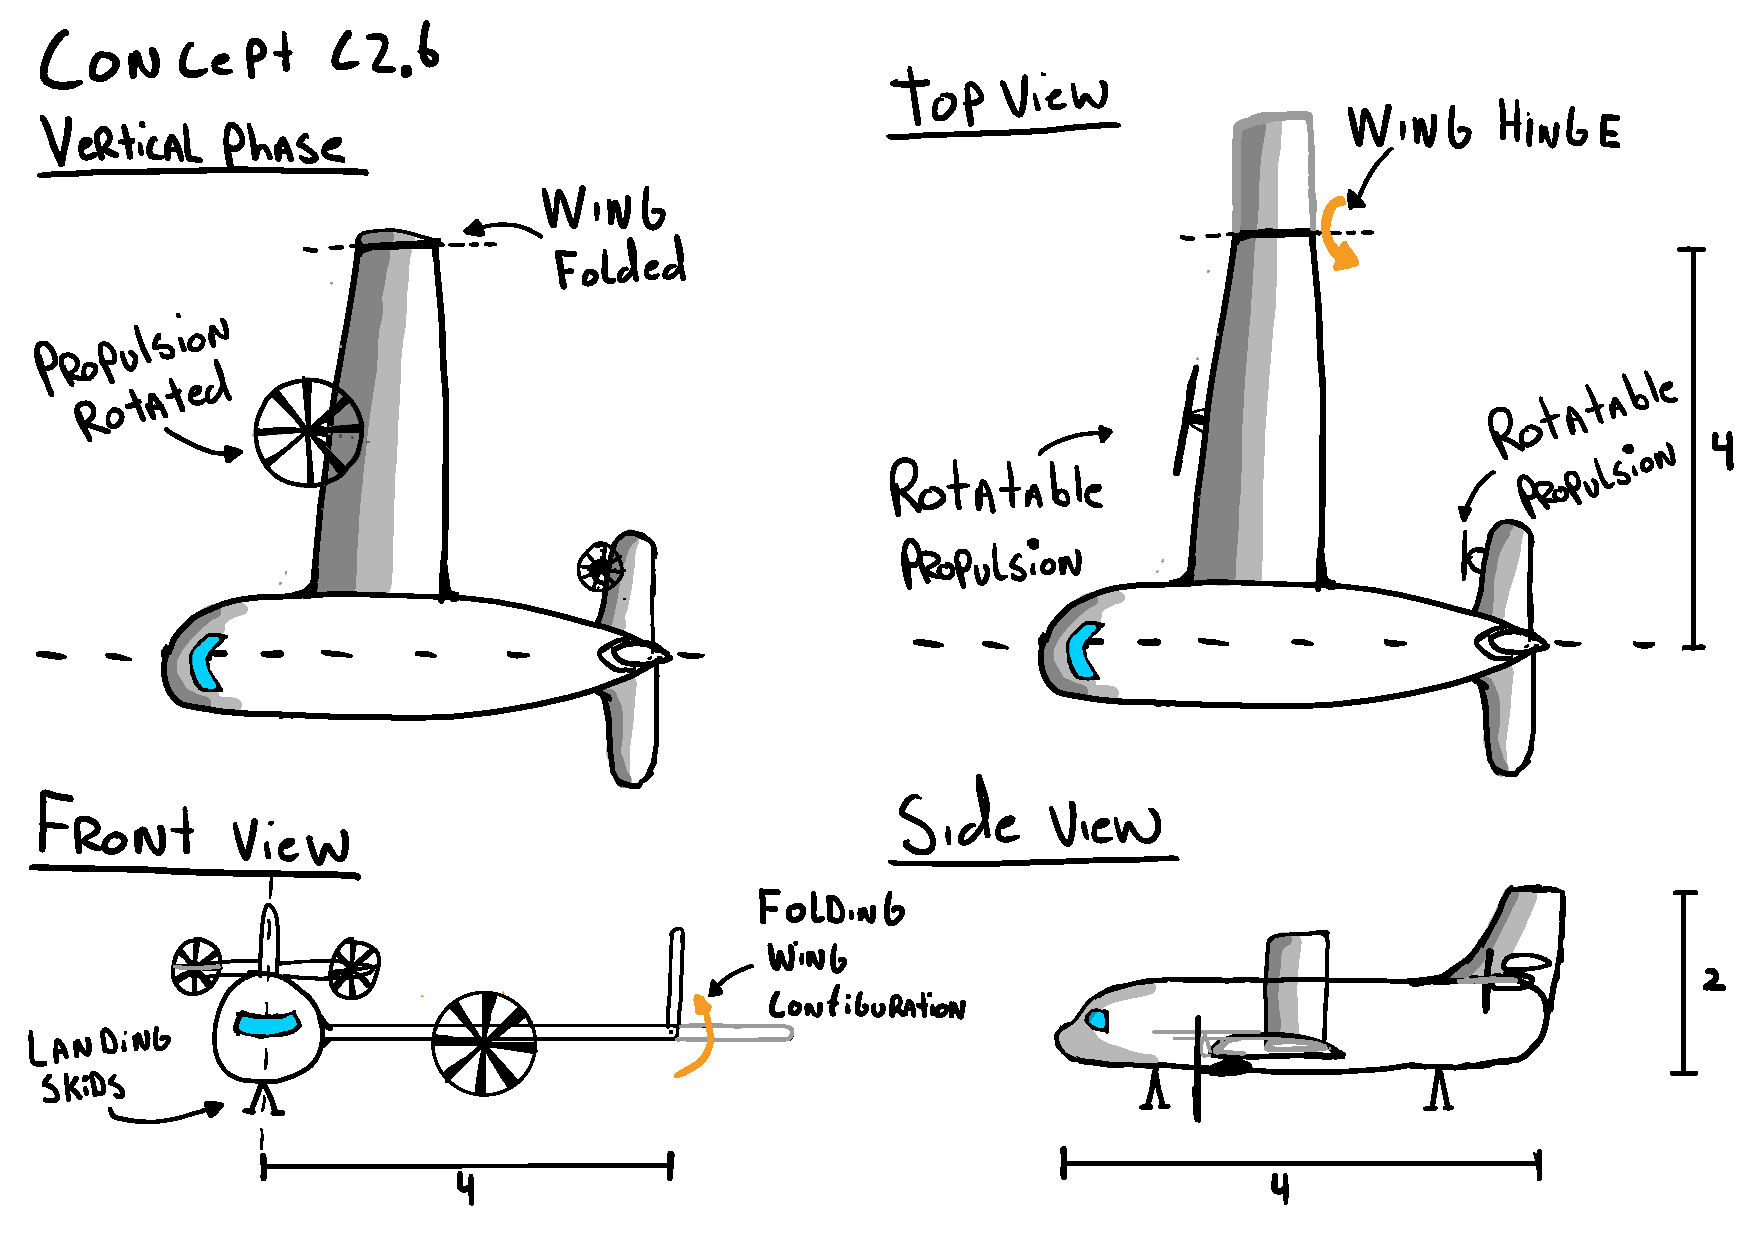
\includegraphics[width=1\linewidth]{figures/Concepts/Concept C2.6 v3.pdf}
    \caption{Concept \newtag{C2.6}\label{C:Folding-Wing}: Folding Wing}
    \label{fig:ConceptC2.6}
\end{subfigure}
\vrule
\begin{subfigure}[b]{0.49\textwidth}
    \centering
    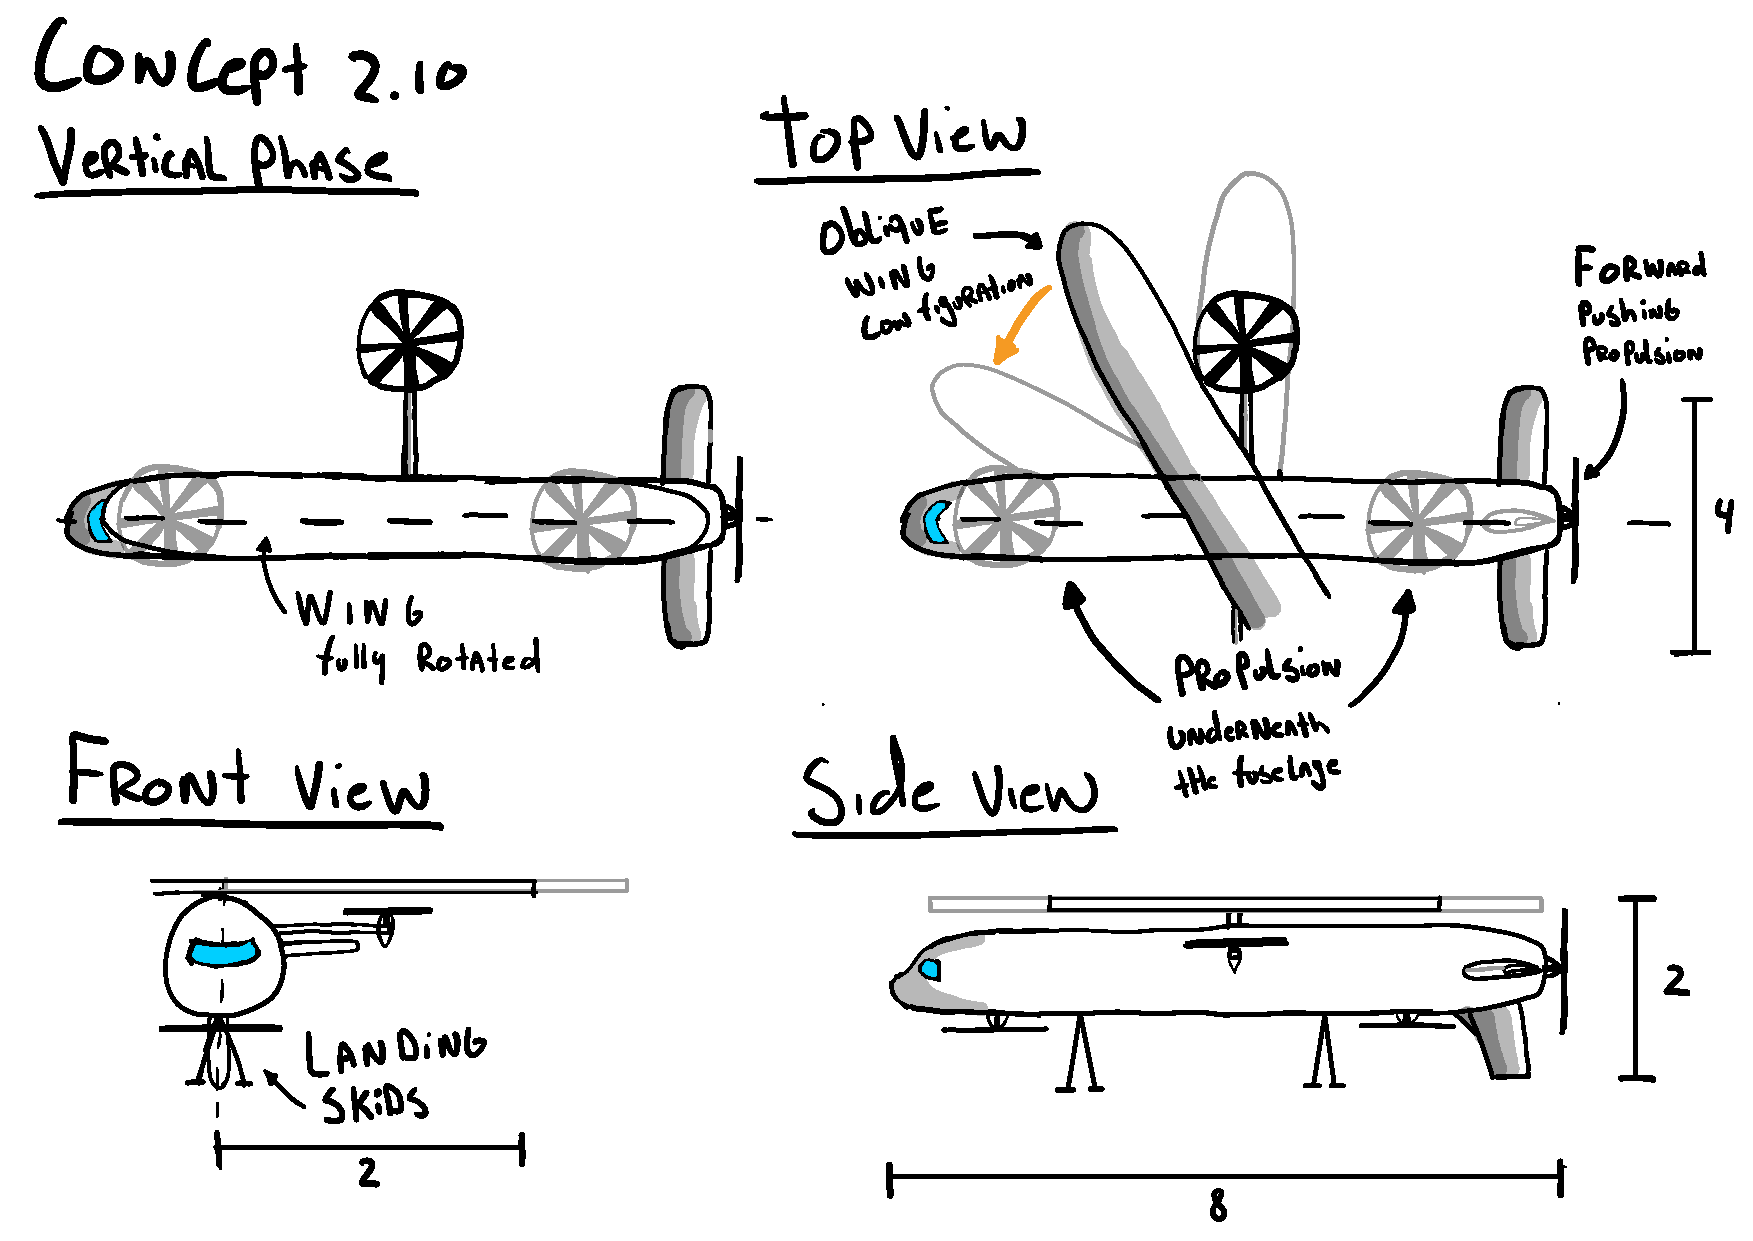
\includegraphics[width=1\linewidth]{figures/Concepts/Concept C2.10 v3.pdf}
    \caption{Concept \newtag{C2.10}\label{C:Variable-Skew-Quadplane}: Variable Skew Quad Plane}
    \label{fig:ConceptC2.10}
\end{subfigure}

    \caption{Concept sketches}
    \label{fig:Concept_sketches}
\end{figure}

\section{Concept C1.7 Exclusion from Trade-off}
Initially, Concept C1.7, the folding wing with engines placed inside of the wing, was also part of the concepts considered for the trade-off.
However, before performing the preliminary sizing that shall be done in the next chapter, it is important to analyse the design concepts critically to ensure the feasibility of the concepts.

On a closer inspection of Concept C1.7, it was determined that, most likely, the concept will be very difficult to design for stability due to the close proximity of the CG to the engines situated on the wing (due to the added weight in the wing area).
The engines situated on the empennage have a large moment arm and, therefore, a large moment that would be generated during the cruise. Keeping the wing engines operating would most likely be necessary to ensure stability during flight.
Moreover, due to the close proximity of the wing engines to the cg as seen in \Cref{fig:engine_in_wing}, the thrust required to be generated by the engines would also be very high.
Therefore a reduction in surface area of the wing occurs, as well as disturbance in the airflow over the wing (\Cref{fig:turbulence_above_wing}).

The engines would also operate near maximum power throughout the flight, leading to energy loss.
Thus, aerodynamic performance would be reduced, and as such, the design was deemed too complex and inefficient and consequently excluded before the trade-off.
\begin{figure}
    \centering
    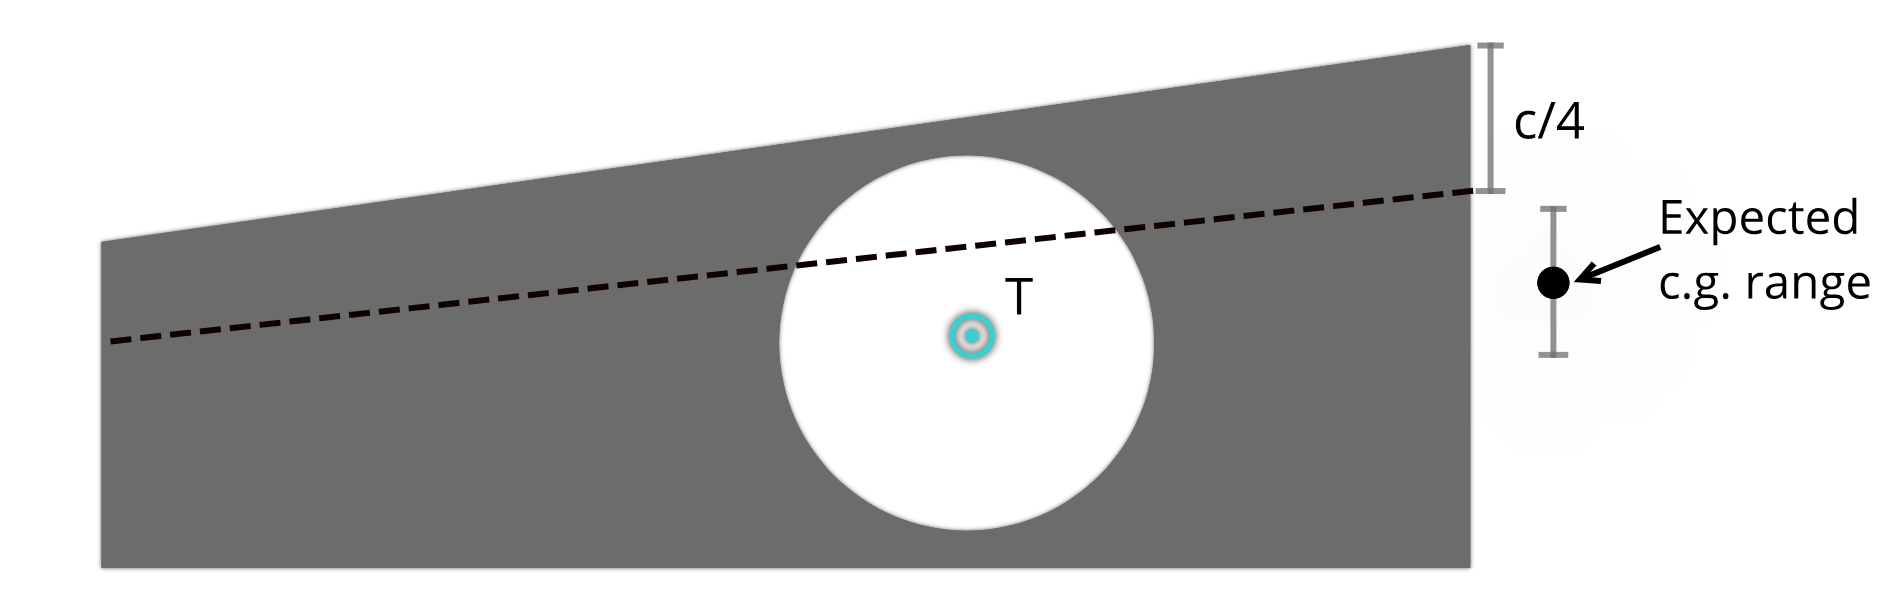
\includegraphics[width=0.7\linewidth]{figures/engineinwing.png}
    \caption{CG position relative to the engine}
    \label{fig:engine_in_wing}
\end{figure}
\begin{figure}
    \centering
    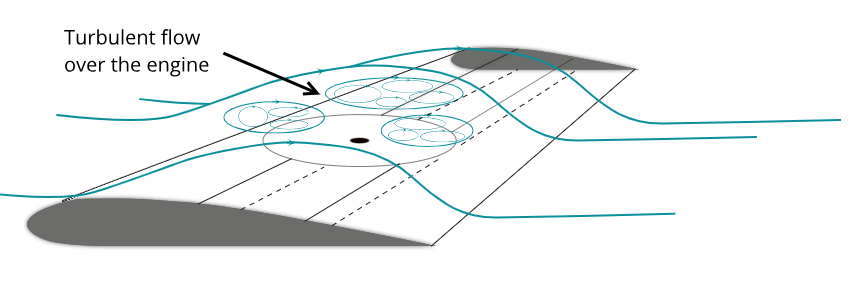
\includegraphics[width=0.7\linewidth]{figures/turbulent.png}
    \caption{Airflow turbulence due to wing propulsion}
    \label{fig:turbulence_above_wing}
\end{figure}
